\documentclass{article}
\usepackage{matheader}
\usepackage{logiccircuits}

\graphicspath{{./res/}}

\begin{document}
	\noindent\begin{tabularx}{\textwidth}{l >{\centering\arraybackslash}X r}
		{Liam Hillery} & {\LARGE \textbf{Project Proposal}} & \today\\
		{\footnotesize {COS 482}} & {\footnotesize {YouTube Metadata Analysis}} & \\\hline
	\end{tabularx}\\
	
	For my project, I plan to analyze the performance of popular YouTube Videos
	across the coming few weeks to generate a dataset, which I will perform some
	analysis on using ML (for text and images) and some cursory data visualization
	for statistics such as views, likes, and comments across many categories and
	tags.

	\begin{figure}[h]
		\center
		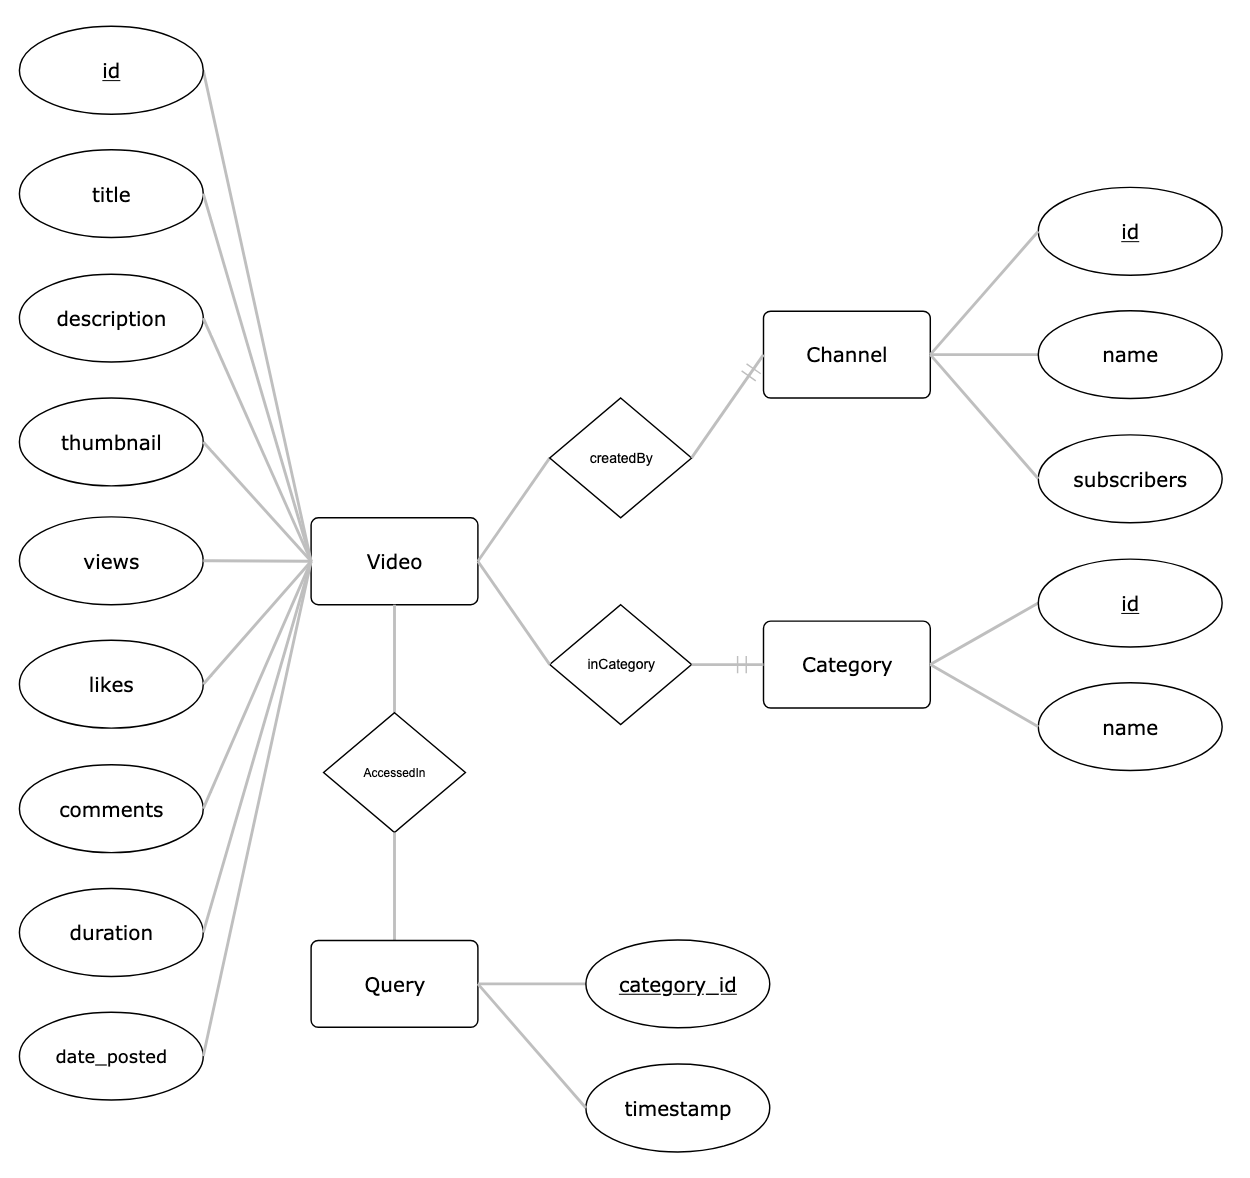
\includegraphics[width=.5\textwidth]{Draft ER Diagram.png}
		\caption{A Draft ER Diagram for the project's SQL Database (not finalized)}
	\end{figure}

	Using the Youtube API, I will collect the 200 most popular videos (both for
	each category and overall) at a set time every day for $\sim$30 days. These data
	(thumbnails, titles, descriptions, interaction counts, etc.) will be stored in
	a PostgreSQL database. Affter this period, I expect to have ~6000 observations
	for each category at which point I will attempt to draw some conclusions. I
	will certainly attempt regression using a CNN trained on the thumbnail data,
	and I will look into NLP systems for the video titles. Because this is a
	historically difficult problem to solve (since video performance is not simply
	a function of title and thumbnail), I don't expect to find very strong
	correlations.
\end{document}